\section{Présentation des outils}
  Pour réaliser notre programme, il faut des outils logiciels.
  Voici une liste exhaustive des outils dont nous avons besoin, et le 
  nom ainsi que la description de ceux que nous avons choisi : 
    \begin{description}
      \item[Un ordinateur] : celui d'Aliaume 
      \item[Un langage de programmation] : nous avons choisi le Vala. Ce langage est en réalité un
        un méta-langage, un traducteur le transforme en un véritable langage de programmation : le C.
        Le C a des avantages, comme la rapidité, et des inconvénients, comme l'insécurité. Le Vala est une 
        surcouche qui permet de simplifier et de clarifier le code, en utilisant des paradigmes de programmation
        que le C n'a pas à travers une bibliothèque nommée GObject, écrite en C.
      \item[Une bibliothèque pour afficher des pixels à l'écran] : nous avons choisi la SDL, qui est une bibliothèque pour le C qui permet d'afficher des pixels à l'écran. Elle est plutôt basique, et par la même très simple. On peut donc faire tout ce que l'on veut … si l'on y met le temps de réfléchir pixel par pixels.
    \end{description}
  
  Ces choix ont été fait pour des raisons de performances, mais aussi parce que le C est un langage qui est éprouvé, et dont les vices sont tous connus. Idem pour la SDL. Tous deux sont très bien documentés. Mais, aussi parce que nous avions déjà utilisé ces outils auparavant.

\section{Programmer le contexte}
  À partir du cahier des charges de la première partie, nous savons déjà comment mettre en place tout ce qui 
  n'est pas la simulation en elle-même. Car au départ, il n'y a pas encore d'expériences, ni de résultats, on ne peut donc que réaliser ce dont on est sûr d'avoir besoin. Malheureusement, dans la plupart des cas, c'est la chose de plus complexe à réaliser.
  Par exemple, il faut créer un menu, c'est évident. Or la SDL ne propose rien de tel. Nous allons donc créer notre propre menu, de manière à pouvoir le modifier facilement au cours du développement et le réutiliser dans des programmes ultérieurs. Le menu est en fait un «~module~». L'idéal dans la programmation de nos jours, est non pas d'avoir le code avec le moins de lignes possibles, mais le code le plus lisible et le plus modulaire. Chaque module doit être indépendant des autres, être facilement modifiable et extensible.
  Voici la liste des modules qu'il faut absolument créer : 
  \begin{itemize}
    \item Le menu
    \item La boite de pétri
    \item La cellule
    \item L'affichage\footnote{Qui simplifie l'utilisation de la SDL, par exemple une fonction «~dessineCellule~» qui exécute automatiquement une liste d'instruction SDL}
  \end{itemize}
  
  Dans chaque module, il y aura différents éléments : 
    \begin{itemize}
      \item Des fonctions
      \item Des variables gobales
      \item Des Classes ou des Structures
    \end{itemize}
  Une classe ou une structure est un patron, une définition formelle d'un nouveau type.
  Après les types classiques comme les nombres ou les lettres, on a la possibilité de créer
  des combinaisons de type (on peut aussi combiner des structures). Tout ceci est définit 
  clairement dans l'annexe \ref{DefStruct} pour les structures, et \ref{DefPOO} pour les
  classes.
  
  Il faut impérativement que chaque module soit bien configurable, adaptable, réutilisable et modifiable facilement, car nous n'avons pour l'instant encore aucune idée des valeurs exactes de la simulation, il faut donc prévoir tous les cas impérativement.
  
  \begin{figure}[H]
		\centering
		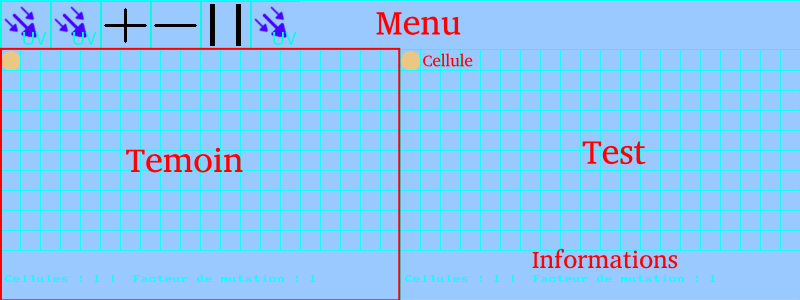
\includegraphics[width=20em]{Images/capture.png}
		\caption{Première vue du programme}
	\end{figure}


\section{Simulation et boucle principale}
  La simulation ne doit s’arrêter que quand on la quitte. On sait donc déjà qu’il y aura une boucle
presque infinie au centre du programme, afin d’éxécuter chaque action qui fait partie d’un cycle de
simulation. On peut donc imaginer une boucle principale de cette manière : 
\begin{figure}[H]
	\centering
	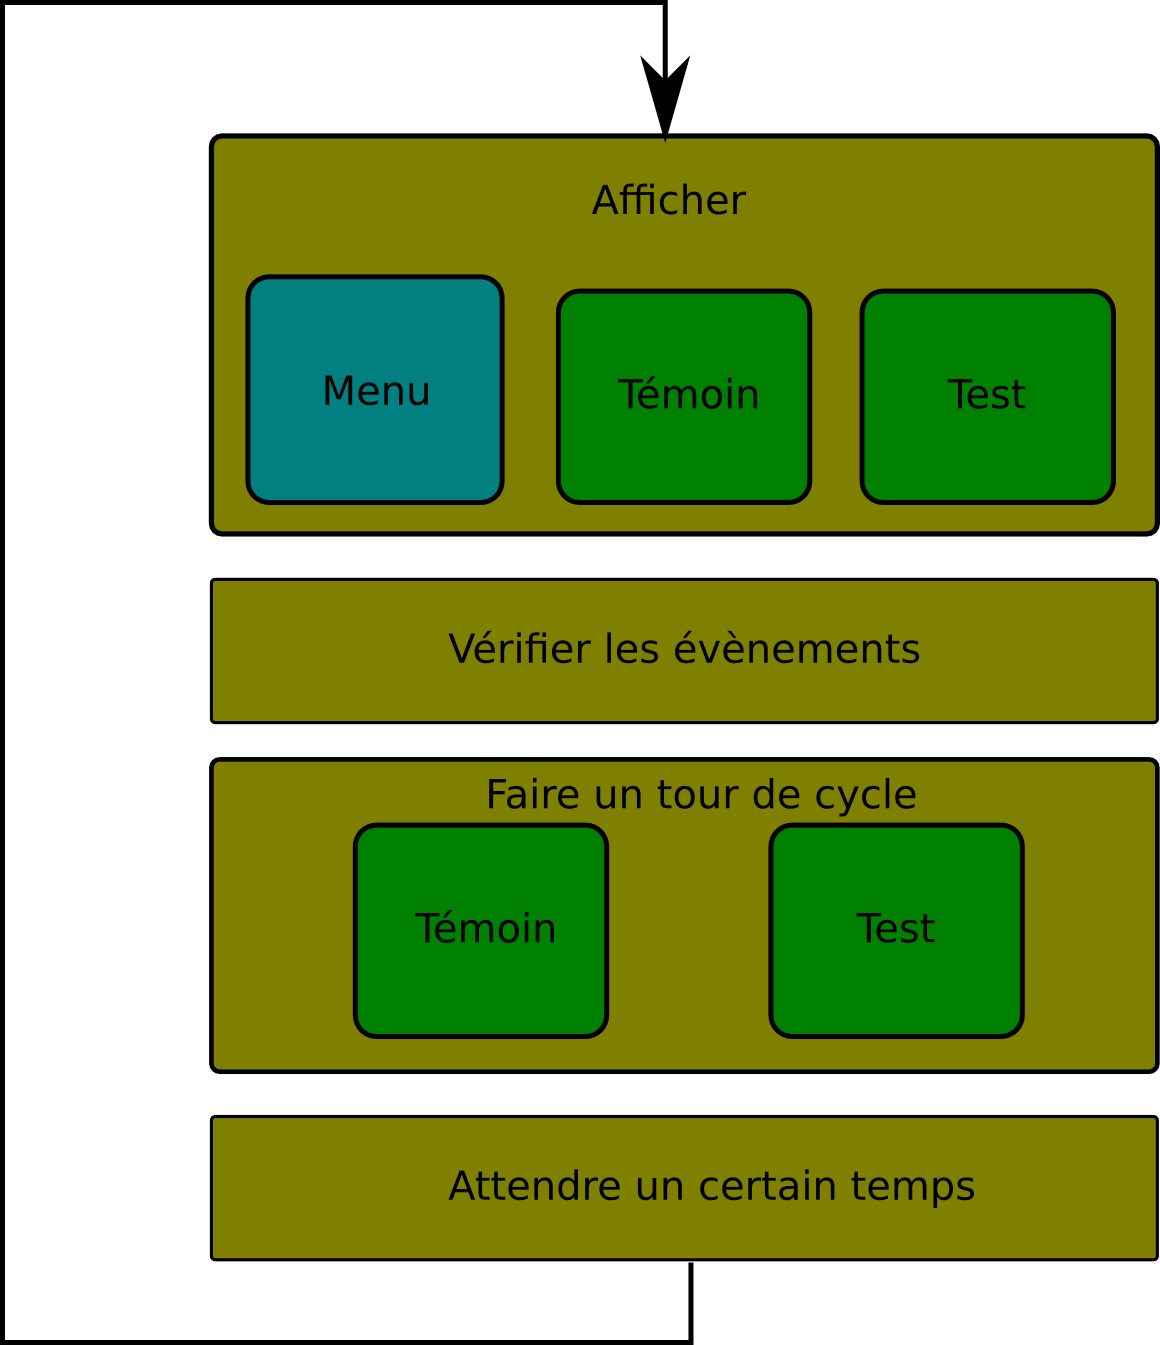
\includegraphics[width=26em]{Images/boucle_naive.png}
	\caption{Une première idée de boucle}
\end{figure}

\begin{description}
	\item[Afficher] : Dessiner le menu, la simulation témoin, la simulation test, et tout ce qu'ils contiennent sur l'écran
	\item[Vérifier les évènements] : récupérer le premier évènement produit et le traiter
	\item[Faire un tour de cycle] : exécuter\footnote{C'est un terme volontairement vague, à ce stade, on ne sait pas encore exactement ce que la simulation va faire} un tour de cycle pour la simulation témoin et la simulation test
	\item[Attendre] : Pour que la simulation soit plus constante, sans cela elle ira aussi vite que possible, et donc sera irrégulière en fonction de la densité de calcul
	\item[Recommencer] : jusqu'à ce que l'on ai demandé de quitter (géré dans les évènements)
\end{description}

On peut imaginer une vision moins naive de cette boucle en divisant les différentes actions en différents processus distincts. Cette méthode est très utile car les processus s'exécutent en parallèle ou presque\footnote{C'est le système d'exploitation qui se charge de leur répartir du temps de calcul, ils ne sont donc pas vraiment en parallèle, sauf avec les ordinateurs récents qui ont plusieurs unités de calcul (processeurs)}. Ceci permet d'avoir une 
vitesse d'affichage constante, par exemple 30 images par secondes, une vitesse d'exécution des simulation différente et une boucle qui gère les évènements avec une vitesse encore différente.

\begin{figure}[H]
	\centering
	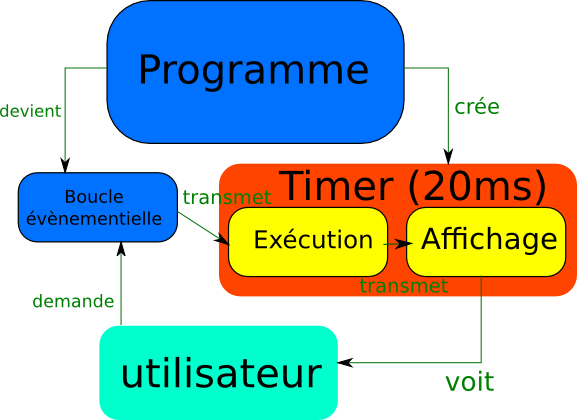
\includegraphics[width=26em]{Images/fonctionnement_programme.png}
	\caption{Fonctionnement du programme}
\end{figure}

Bien sûr il faut que les processus puissent communiquer entre eux. Et cela pose problème, étant donné qu'ils s'exécutent en parallèle, et qu'on ne sait pas lequel va être lancé en premier. On peut leur faire partager des variables, mais il faut bien vérifier qu'elle soit à jour, et éviter les modifications simultanées par deux processus d'une même variable ! C'est la seule difficulté rencontrée par la séparation en plusieurs processus, la solution a été d'utiliser des verrous : avant de faire une action on demande un verrou sur cette variable et on est sur que personne d'autre que nous ne peut la modifier, ensuite on libère le verrou, et c'est un autre processus qui prend possession de la variable. Cette méthode peut entrainer des ralentissements, des décalages, mais nous ne partageons que 2 variables, donc normalement, il n'y a pas de raisons que ces ralentissements soient visibles.


\section{Rectangle, la base}
  Nous savons que la majorité des éléments de la simulation seront affichés à l'écran.
Or pour afficher quelque chose sur une surface, il faut un certain nombre d'informations : 
\begin{itemize}
  \item Position $(x,y)$ sur l'écran
  \item Taille $(w,h)$
\end{itemize}

Nous dessinerons uniquement des rectangles, pour des raisons de simplicité, et parce que nous n'avons pas besoin d'autres formes géométriques dans notre simulation\footnote{En effet, même si on définit les cellules comme des cercles, pour afficher une image, il faut le rectangle de la taille de l'image, même si l'image elle même est un rond sur fond transparent}.

Avec ces variables, on peut ajouter plusieurs méthodes qui seront utiles :
\begin{itemize}
  \item déplacer($x$,$y$); $\rightarrow$ redéfinit la position $(x,y)$
  \item move ($x$,$y$); $\rightarrow$ effectue une translation par le vecteur $(x,y)$
\end{itemize}


Nous avons donc notre première classe : \texttt{Rectangle}, qui sera la base pour afficher des objets à l'écran.


\section{L'exemple du menu}
  
L'exemple du menu étant simple et parlant, nous montrerons comment nous avons pensé 
ce module. Dans un menu, il y a des boutons. Donc il faut un objet Menu\footnote{De manière à être 
utilisable dans d'autres programmes, ou pouvoir faire plusieurs menus}, et un objet Bouton. Un Bouton est un objet affiché à l'écran, il faut donc le faire hériter de Rectangle, un objet Menu a une position sur l'écran, il faut donc aussi qu'il hérite de Rectangle.

De cette manière on a maintenant des classes comme ceci :
\begin{figure}[H]
	\centering
	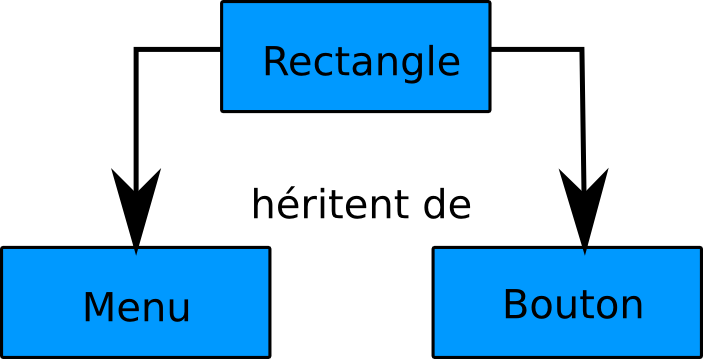
\includegraphics[width=26em]{Images/heritage_menu.png}
	\caption{Représentation de l'héritage des classes}
\end{figure} 
  
\subsection{Bouton}
	Bouton est une classe qui hérite de Rectangle, mais elle apporte son lot de nouveautés, à savoir tout ce qui est relatif au bouton : 
	\begin{itemize}
		\item une image pour le bouton normal
		\item une image pour le bouton activé
		\item une variable pour savoir si le bouton est activé
		\item une variable de type ennumération\footnote{Voir annexe \ref{DefEnum} sur les énnumération, qui parle du menu en exemple} pour savoir l'action qu'il entraine
	\end{itemize}
	
	Le bouton lui-même n'a pas vraiment de fonctions, tout le code se trouvera dans le gestionnaire des boutons, le Menu. Mais avant de parler du menu, il faut définir les actions, or nous ne savons pas encore lequelles il y aura, nous allons donc créer une énnumération, qui sera traitée dans la boucle des évènements. Ajouter une action demandera d'ajouter un item à l'énumération, et un traitement de cet item dans la boucle évènementielle.
	
\subsection{Menu}
	Le menu gère les boutons, son code n'est pas aussi complexe qu'on pourrait se l'imaginer, il contient un tableau de boutons, une fonction «~affiche~» qui affiche le menu et une fonction «~recupBouton~» qui retourne le bouton à la position du curseur.
	
	La seule difficulté réside dans le fait de dessiner correctement les boutons, et au bon endroit. Pour cela il faut savoir que l'écran de la SDL se comporte comme un repère orthonormé, à ceci près qu'il a pour origine le coin haut gauche de la fenêtre, et que son axe des Y est inversé par rapport aux graphiques habituels : 
	
	Après ça, il faut aussi savoir que le menu a une position, donc quand on place un Bouton, il faut le placer en fonction de la position du menu, et en fonction de la taille d'un Bouton. La méthode suivante est utilisée : 
	« $boutons.push(new Bouton (image,action, TAILLLE_BOUTON * numero_bouton + menu.x , menu.y,image_activé));$ ». Ce code se suffit, quand on crée un bouton, on lui donne deux images, une action, et la position du bouton vaut celle de la simulation, plus $N$ fois la largeur d'un bouton en $x$, en fonction du numéro du bouton.
	
	C'est bon, nous avons un menu fonctionnel, reste à connecter tout cela avec la boucle évènementielle et c'est terminé. Nous ne parlerons pas de la boucle évènementielle, car elle est en réalité simple. Globalement elle demande si le curseur a cliqué, si oui où. Après elle regarde sur quelle partie du programme le curseur est positionné, et un système de conditions décide de ce qu'il faut faire. Ce code n'est pas intéressant, simplement parce que c'est une suite de conditions imbriquées sans grande complexité.

  
\section{Conclusion}
  Nous avons maintenant à travers quelques exemples précis décrit toute la mise en place des éléments périphériques à la simulation. Éléments indispensables, mais qui ne concernent pas directement le projet final. Nous allons donc pouvoir passer aux recherches sur la simulation elle-même, qui vont dégager des affirmations et prédicats pour coder la simulation ensuite.

    
     
